\section{Page--Wootters and detector absorption models}\label{sec:absorption+pw}

The detector absoption model in \cite{RuschhauptAbsorption} is not originally
based on the notion of quantum relational time. It's ``ordinary quantum mechanics''
in the sense that states are in $\hilb{H}_S$ with an external parameter time;
but, contrary to quantum mechanics, the potential can be \emph{complex},
causing the norm of the state vector to not be conserved (in fact, vanishing with time).
In other terms, the evolution is not unitary, even for a pure state.
Specifically, the Hamiltonian is corrected by an anti-hermitian term
that models the detector.

A non hermitian Hamiltonian is justified as a computation method
to simplify the study of some open systems: the evolution of mixed
states is derived without explicit reference to density operators
or master equations, but resolving equations that are formally
identical to those of pure states,
i.e. in terms of
Schr{\"o}dinger equations and wave functions,
with the non-hermitian term in the Hamiltonian
to account for the non-unitarity of the evolution.
%
This is treated extensively in:
  \cite[Ch. 6]{TQM2};
  \cite{Wave-function_approach};
  \cite{HowToResetAnAtom};
  \cite{TheQuantumJumpApproach};
  \cite[\S 8.5.2 ``The `quantum jump' approach to damping: The wave function Monte Carlo approach'']{ScullyZubairy};
  \cite[\S 6.7.1 ``Simulating Quantum Trajectories'']{WallsMilburn}.

The detection-by-absoption model in \cite{RuschhauptAbsorption}
is based on a complex potential that, plugged into the Schr\"odinger equation,
leads to a non-unitary evolution of the state vector
(with loss of normalization).

Specifically, the Hamiltonian $\hat{H}$ is replaced by a $\hat{H} - i\hat{D}$
(with $\hat{D}$ self-adjoint, bounded, positive ---\cite{RuschhauptAbsorption})
and, consequently:
\begin{equation}\label{eq:schrod_complex_pot}
  \hat{H} \ket{\psi(t)} = i\hbar\dv{t}\ket{\psi(t)} +i\hat{D}\ket{\psi(t)} \text{.}
\end{equation}

One may wonder whether a proper, normalized Page--Wootters ``position-time wavepacket''
(as described in \S\ref{sec:properpw})
can be used to describe \emph{the event of being detected} (or being absorbed).
It's expected to be peaked around the time when the absorption by the detector is maximum.

In the detector model of \cite{RuschhauptAbsorption}, the detection
by absorption
corresponds to the \emph{decrease} in norm of the wavefunction.

Therefore we expect the following relation to be true:
\begin{equation}\label{eq:pwkiukas}
  \abs{\phi(t)}^2 = -\dv{t}\norm{\psi_{\text{Kiukas}}(t)}^2 \text{,}
\end{equation}
both sides of which indicate probability of arrival at time $t$.
Here the function $\phi$ of time $t$ has to be intended in the sense of
\eqref{eq:pwphi}.

Interestingly, \cite{RuschhauptAbsorption} provides a solution of \eqref{eq:pwkiukas}.
Despite being not based on the Page--Wootters model, eq. 9 therein
equates the squared norm of a ``time representation'' wavefunction
to the opposite derivative of the squared norm of the ``absorbed wavefunction''.
It reads:
\begin{quote}
  We will associate with any wave function $\psi \in \hilb{H}$
  another wave function $\hat{\psi}$,
  which is a function of time, so that
  $\abs{\hat{\psi}(t)}^2$
  is the arrival probability density. In other words,
  $\hat{\psi}$ is a wave function in a time representation. For each
  $t$, $\hat{\psi}(t)$ lies in the original Hilbert space $H$.
\end{quote}
Therefore we ``translate'' $\hat{\psi}(t)$ into $\phi(t)\ket{\psi(t)}_S$
and, consequently, $\abs{\hat{\psi}(t)}^2$ into $\abs{\phi(t)}^2$,
in the language of the Page--Wootters model and within the notation
adopted.

Using eq. 8 in \cite{RuschhauptAbsorption} and translating into our notation we have:
\begin{equation}\label{eq:phi_psi_kiukas}
  \hat{\psi}(t) \eqbydef
  \phi(t)\ket{\psi(t)} =
  \begin{cases}
    \sqrt{\frac{2}{\hbar}} \hat{D}^{1/2} \ket{\psi_{\text{Kiukas}}(t)}_S &\text{ if } t > 0 \\
    0 &\text{ otherwise. }
  \end{cases}
\end{equation}
Where at $t \le 0$ the interaction with the detector is yet to come,
but so it is, as a limit, for small values of $t>0$,
in other terms
$\lim_{t \to 0^{+}} \norm{\hat{D} \ket{\psi_{\text{Kiukas}}(t)}} = 0$, thus avoiding the apparent discontinuity.

% \subsection*{\color{red} TODO}

% {
%   \color{red}
%   Figure out how to connect the above to what follows (or drop or separate if does not apply).

%   \scriptsize{
%     Hint: rather then the ``conspiracy theory''
%     (``I find an imaginary term both here and there'')
%     consider (time of) arrival as in \cite{Maccone:QMOT}.
%     This should bring to a normalized element of $\pwspace$ \dots
%   }
% }

\subsection{Application: two-level system}

In \cite{RuschhauptAbsorption}, an example application of the detector model
is provided for a two-level system.
In Page and Wootters terms,
this would corrspond to a bi-dimensional $\hilb{H}_S$, but a continuous
spectrum of $\hat{T}$ in $\hilb{H}_T$. The paper is \emph{not} based on
the Page--Wootters model, indeed the purpose of this section is a comparison
with such model, using the results of \S \ref{sec:absorption+pw}.

By setting, out of convenience, $\hbar = \omega = 1$
(with $\omega$ the characteristic frequency of the system),
and directly considering the parameters
that minimize the time--energy uncertainty product \parencite{RuschhauptAbsorption},
we have a non-hermitian ``hamiltonian''
$\mathcal{K} = \hat{H} - i\hat{D}$ with
\begin{equation}\label{eq:complexpot}
  \mathcal{K} = \hat{H} - i\hat{D} \repr
    \hbar\omega\left\{
      \left[\begin{matrix}0 & 1\\1 & 0\end{matrix}\right] -
      i \left[\begin{matrix}0 & 0\\0 & \gamma \end{matrix}\right]
    \right\}
\end{equation}
and $\gamma = 2\sqrt{2}$.

We take an initial state of $\ket{0}$
(or $\mqty[1\\0]$ in matrix form).

We then compute, symbolically, the non-unitary evolution
$\ket{\psi(t)} = e^{-i\mathcal{K}t}\ket{0}$
with the aid of \term{SymPy} \parencite{comp:sympy} within a \term{Jupyter} \parencite{comp:jupyter} notebook
(see Appendix \ref{detector-model-kiukas-ruschhaupt-schmidt-werner} for all the details of the calculation).

Simplifying the result in eq. \eqref{eq:sympy:non-unitary-evol}, we have:
\begin{equation}
  \ket{\psi(t)} \repr e^{-\frac{\sqrt{2}}{t}} \mqty[
    \cos{\frac{\sqrt{2}}{2}t} + \sin{\frac{\sqrt{2}}{2}t}& \\
                     -i\sqrt{2} \sin{\frac{\sqrt{2}}{2}t}&
  ] \,\text{.}
\end{equation}

\begin{figure}
  \centering
  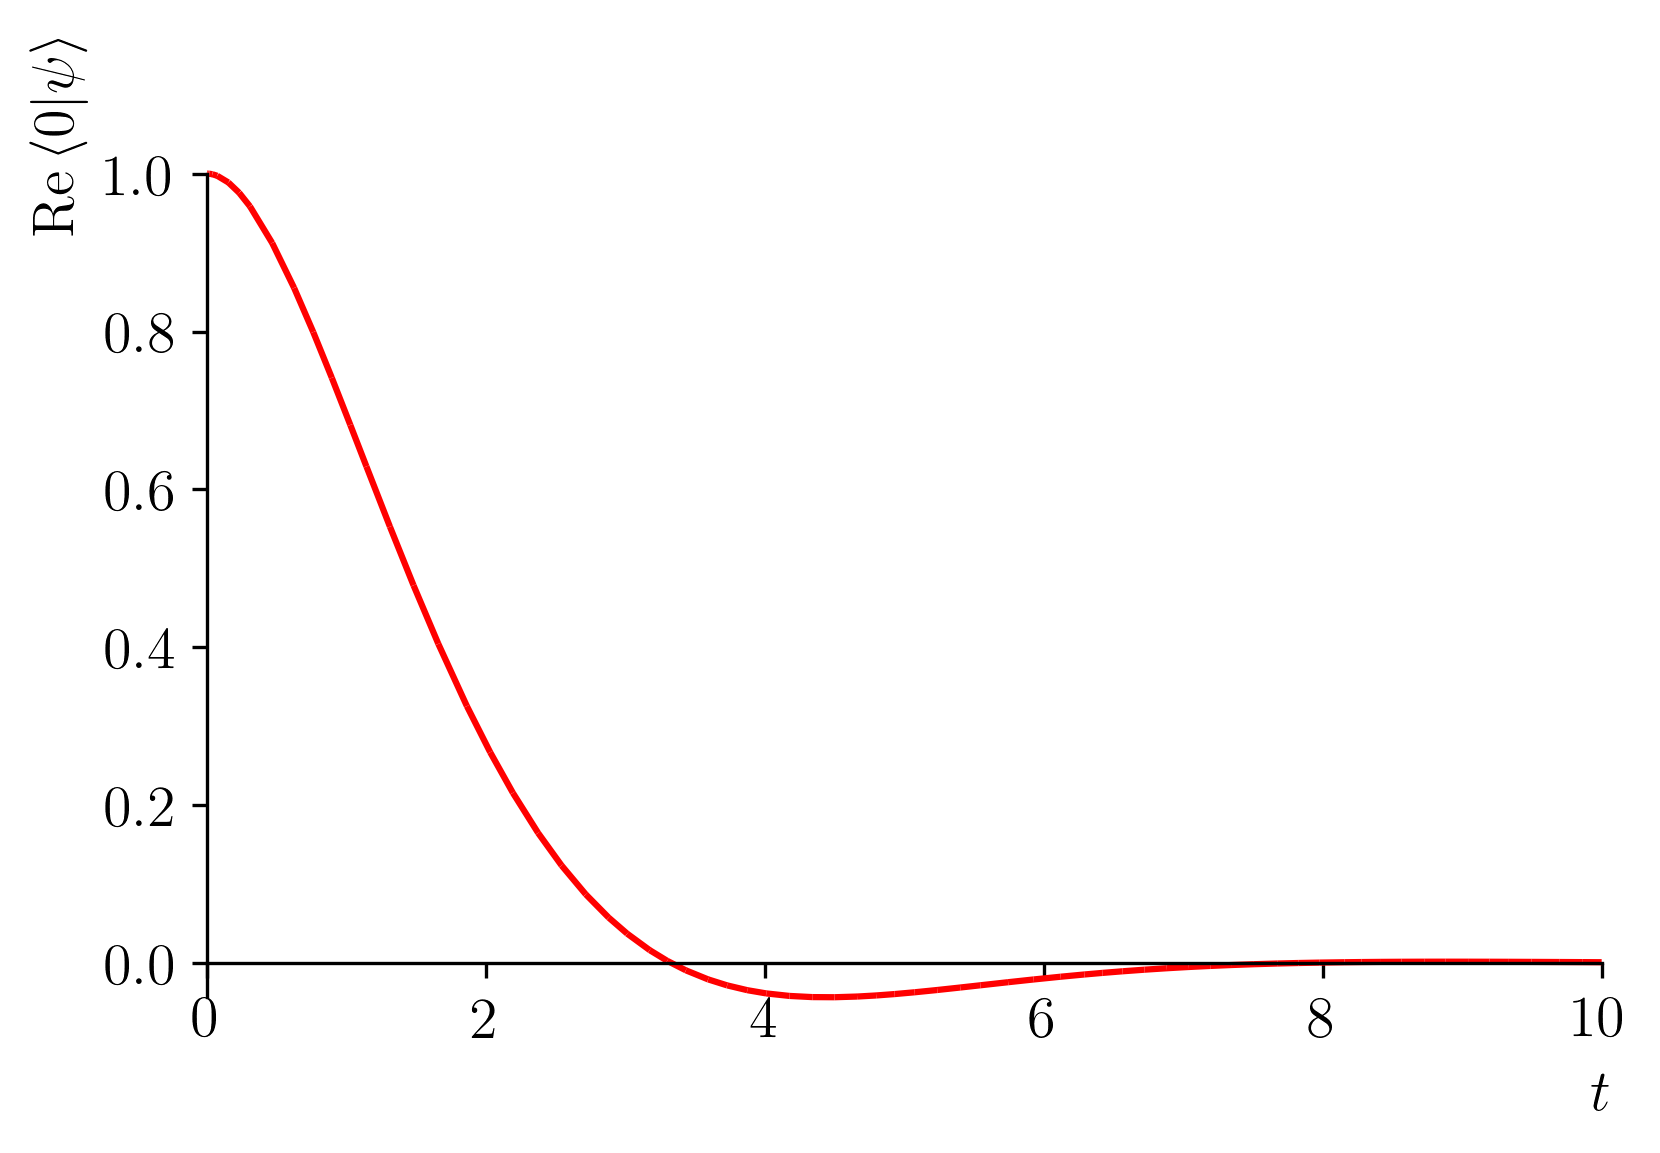
\includegraphics[width=0.49\textwidth]{img/2ldetect/re_psi0_t.png}
  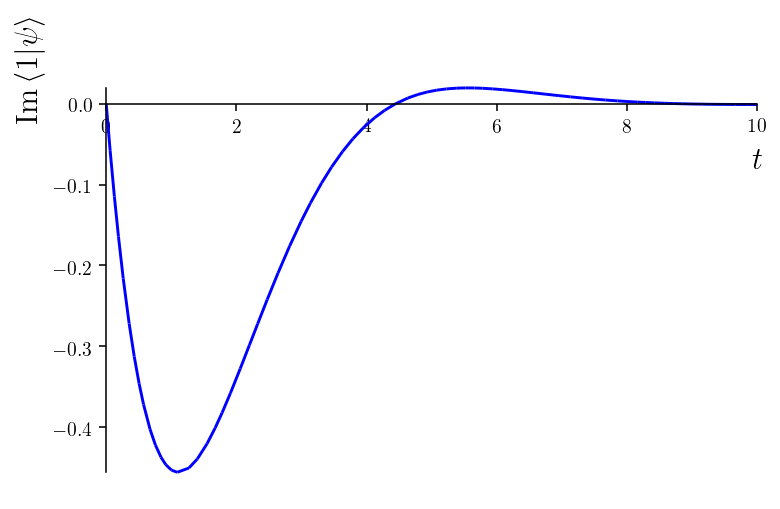
\includegraphics[width=0.49\textwidth]{img/2ldetect/im_psi1_t.png}
  \caption{
    Non-unitary evolution of the absorbed qubit.
    The component along $\ket{0}$ is purely real,
    and the one along $\ket{1}$ is purely imaginary,
    therefore only their their respective parts are plotted.
  }
  \label{fig:absorbed-qubit-components}
\end{figure}

\begin{figure}
  \centering
  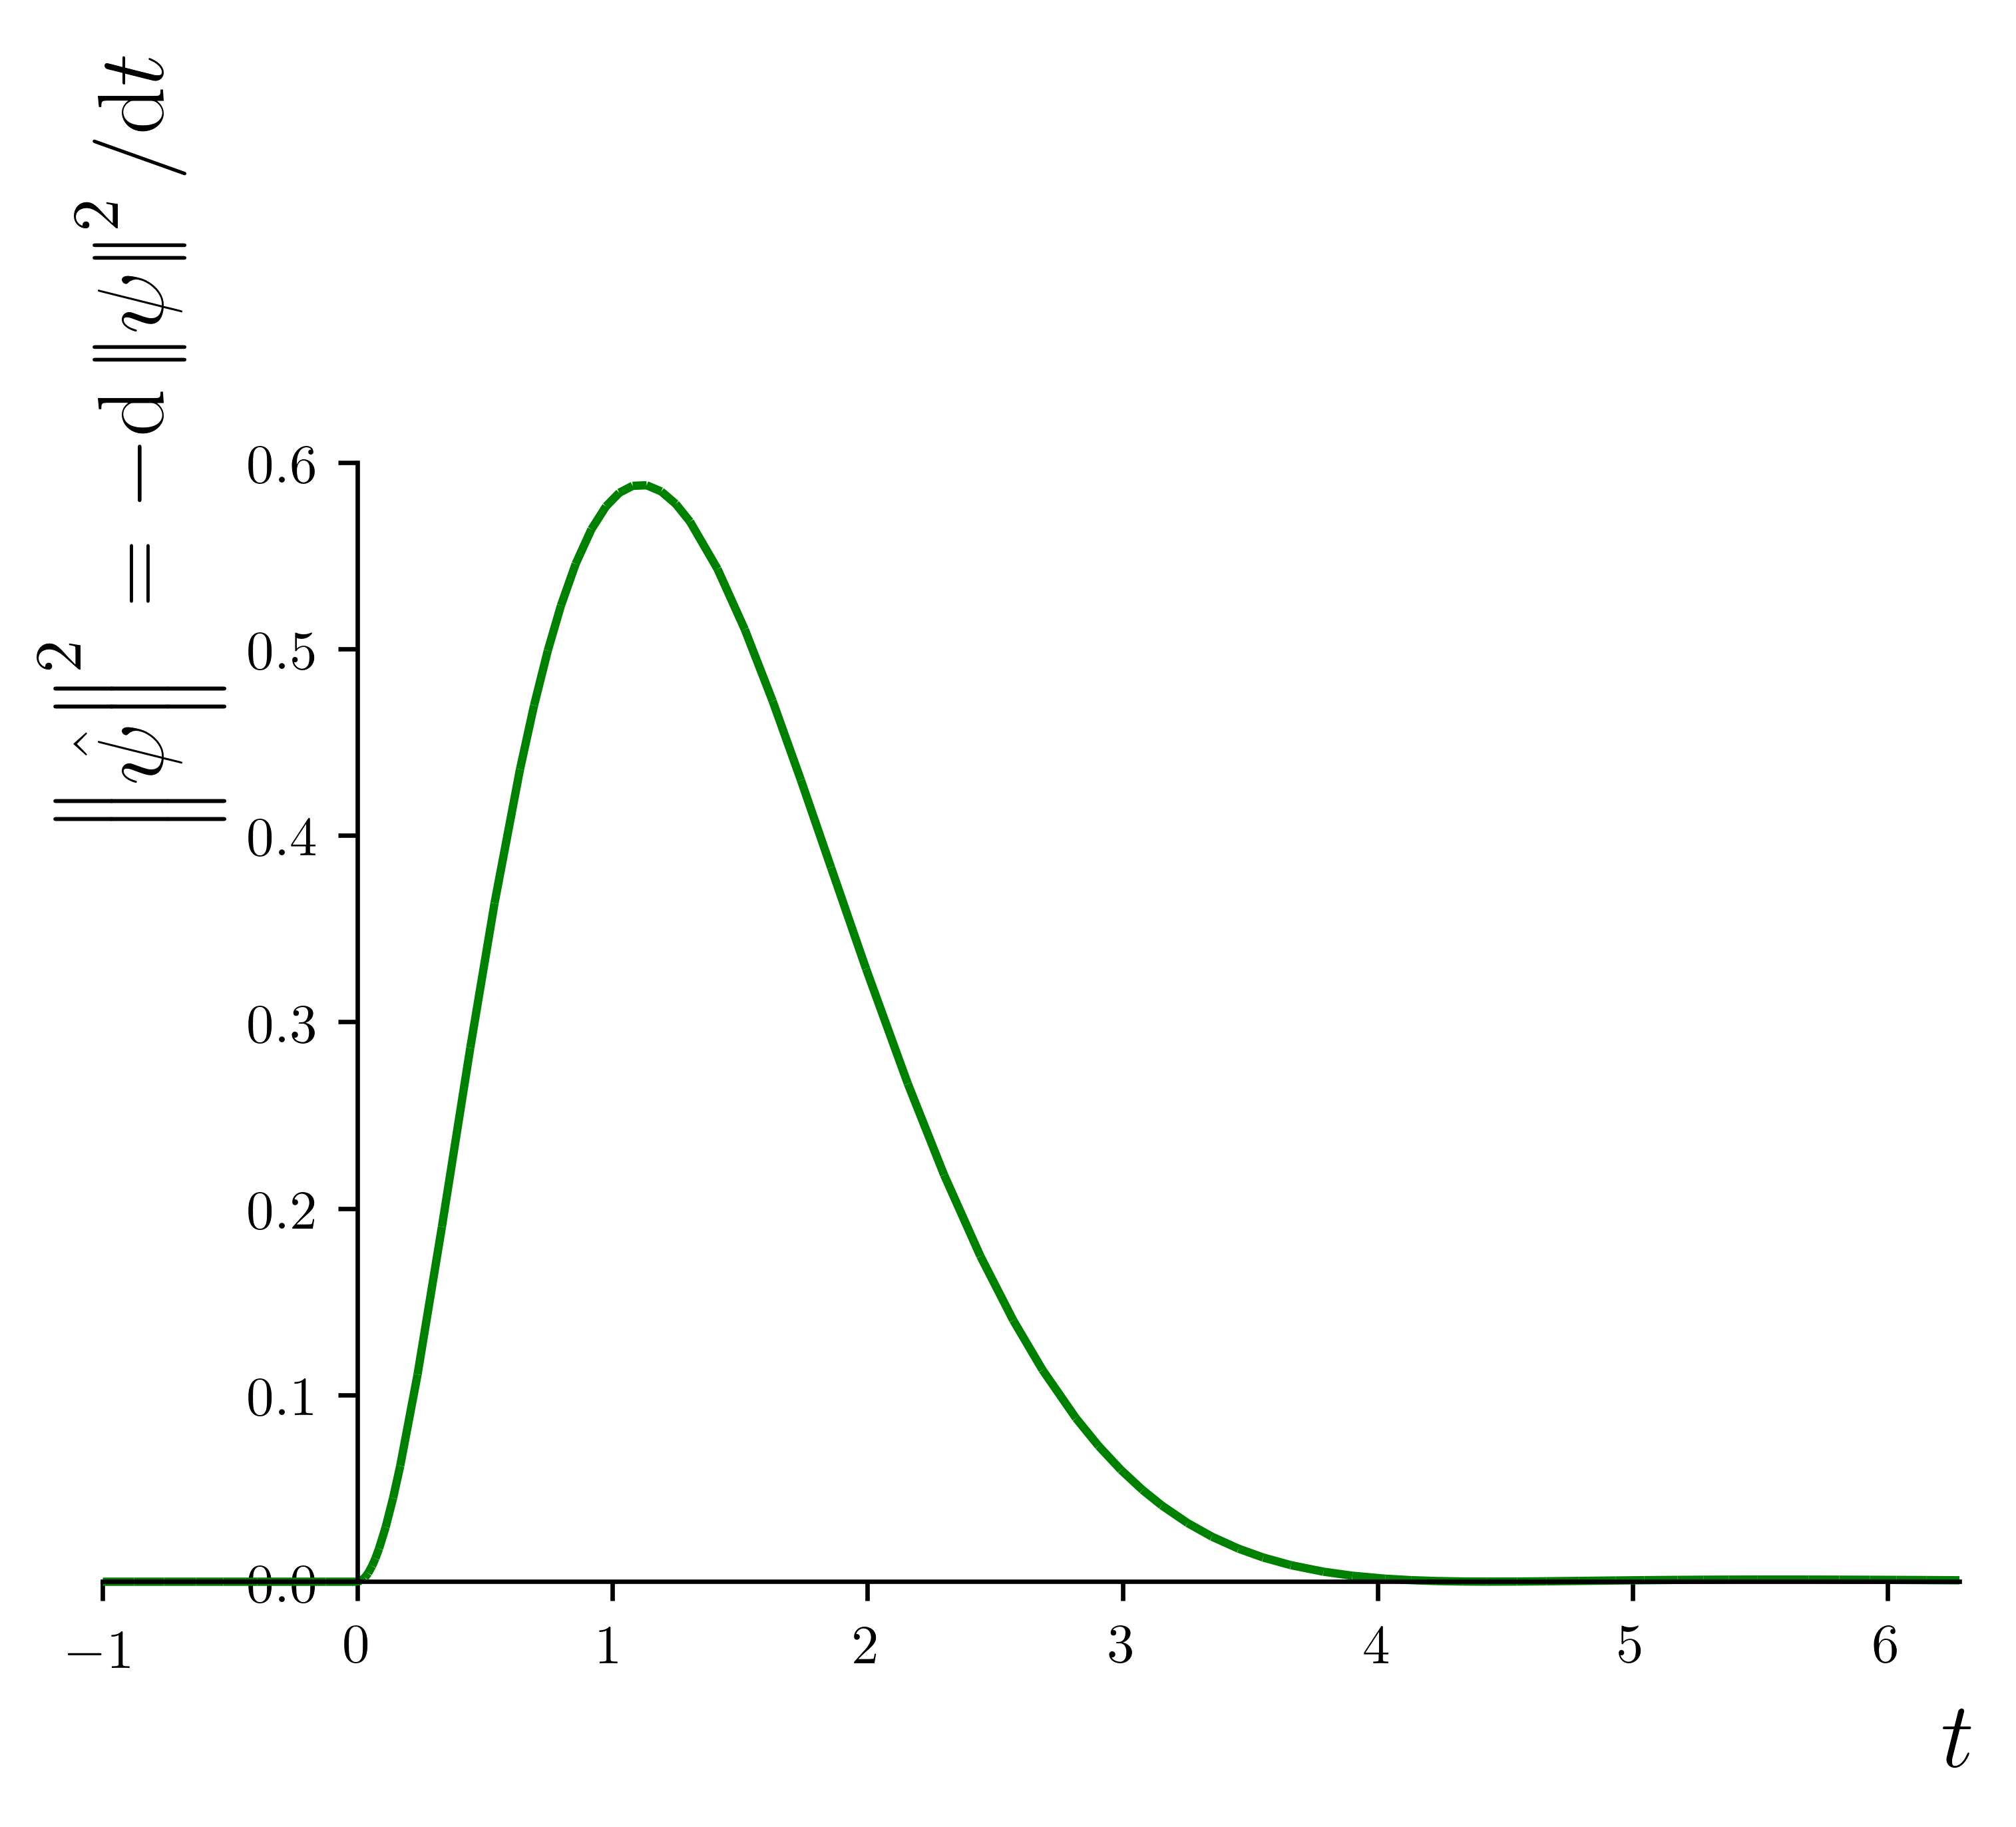
\includegraphics[width=0.49\textwidth]{img/2ldetect/qubit_normalization_loss.png}
  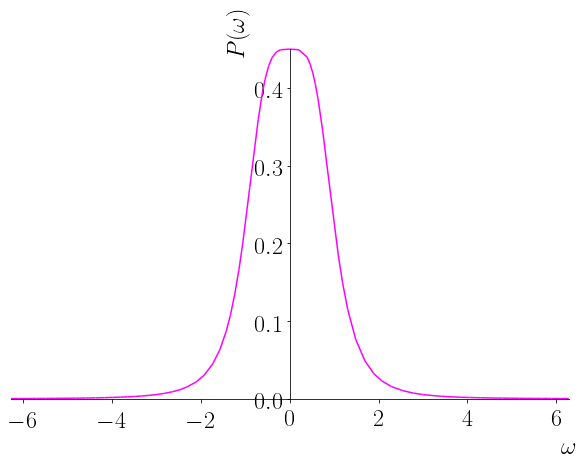
\includegraphics[width=0.49\textwidth]{img/2ldetect/P_omega.png}
  \caption{
    Non-unitary evolution of absorbed qubit.
    \emph{Left}: loss of normalization $-\dv{\norm{\psi}^2}{t}$ (detection probability in time).
    \emph{Right}: detection probability in the frequency domain.
  }
  \label{fig:absorbed-qubit-normalization-loss}
\end{figure}

The ``lossy'' evolution, with the two components of the qubit, is shown in Fig.~\ref{fig:absorbed-qubit-components}.
The loss of normalization $-\dv{\norm{\psi}^2}{t}$, indicating the probability of detection by absorption,
is then derived directly and shown in Fig.~\ref{fig:absorbed-qubit-normalization-loss}.

This yields the \emph{probability} of detection.
One may wonder whether it is possible to derive a corresponding \emph{probability amplitude} vector,
whose squared norm across time is equal to the said probability distribution.\footnote{
  The solution is of course not unique, but one may ask whether such functions would lead
  to quantum interference patterns and other phenomenology which may be subject of further study.
}
Within the framework of \cite{RuschhauptAbsorption}, a ``wavefunction in time'' in such sense
is the $\hat{\psi}$, as in \eqref{eq:phi_psi_kiukas}.
It is computed in detail within the
notebook in Appendix \ref{detector-model-kiukas-ruschhaupt-schmidt-werner}, eq. \eqref{eq:sympy:hatpsi},
simplifying which we obtain:
\begin{equation}\label{eq:analytic:hatpsi}
  \hat{\psi}(t) =
    i 2^{\frac{5}{4}} e^{-\frac{\sqrt{2}}{2}t}\sin(\frac{\sqrt{2}}{2}t) \theta(t)
    \ket{1}
    \text{,}
\end{equation}
with $\theta(t)$ the Heaviside step function.

In general, the operator $\hat{D}$ as in \eqref{eq:schrod_complex_pot}
is such that the eigenspace corresponding to its eigenvalue $0$
is the ``area'' where the detector is not sensitive. Or, in other words,
the linear span of states with zero probability of triggering the detector.
Therefore, when $\hat{D}$ (or its square root) is applied to a state vector,
for example in \eqref{eq:phi_psi_kiukas},
the components in such eigenspace are cut off and the resulting
$\hat{\psi}$, eq. \eqref{eq:analytic:hatpsi} in the example, lies at all times in the ``area of detection''
i.e. it's a multiple of $\ket{1}$ in this case.

The corresponding Page--Wootters (proper) vector of $\pwspace$ is
\begin{equation}\label{eq:hatpsi:pw}
  \Dket{\hat{\Phi}} = \int \dd{t} \ket{t} \ox \hat{\psi}(t) \,\text{,}
\end{equation}
to which the considerations of \S\ref{sec:for-normalized-elements}
and \S\ref{sec:pure-state-approach} in terms of time--frequency
(or time--energy) uncertainty relation apply, with some analogy
to what \cite{RuschhauptAbsorption} does within its own framework
in relation to $\hat{\psi}$ and its Fourier transform.

In that regard, the \eqref{eq:hatpsi:pw} can be reformulated
\begin{equation}
  \Dket{\hat{\Phi}} = \int \dd{\omega} \ket{\omega} \ox \mathcal{F} \hat{\psi} (\omega) \,\text{,}
\end{equation}
where it's
\begin{equation}
  \mathcal{F} \hat{\psi} (\omega) = - \frac{\sqrt[4]{2} i}{\sqrt{\pi} \left(- \omega^{2} + \sqrt{2} i \omega + 1\right)} \ket{1}
\end{equation}
---see notebook up to \eqref{eq:fhatpsi1_omega} for details.

Taking the squared modulus, a probability distribution over angular frequency
(or, equivalently, energy) is obtained:
\[
  P(\omega) = \frac{\sqrt{2}}{\pi \left(\omega^{4} + 1\right)}
  \,\text{.}
\]
See Fig. \ref{fig:absorbed-qubit-normalization-loss}, \emph{Right}.

\subsubsection{
  (Non-unitary) evolution without evolution:
  plugging the complex potential in the \emph{discrete} Page--Wootters model
}

Similarly to what seen in \S \ref{sec:building-the-discrete-pw-clock}, we build
the clock by defining ---and representing in a convenient basis---
the time operator and the corresponding frequency operator:
\begin{align}
  \hat{T} \repr \frac{2\pi}{N}
  \begin{pmatrix}
    0           &       &       &       \\
                &1      &       &       \\
                &       &\ddots &       \\
                &       &       &N-1
  \end{pmatrix}
  &&
  \hat{\Omega} = \frac{N}{2\pi} F^{}_{N} \hat{T} F^{\dagger}_{N} \, \text{,}
\end{align}
where $F$ is, again, the discrete Fourier operator of order $N$.

Next we define the Wheeler--DeWitt operator $\mathbb{J}$ as in
\eqref{eq:pwHamiltonian}, but $\hat{H}_S$ is replaced by the non-hermitian
Hamiltonian of the detector model
$\mathcal{K}_S = \hat{H}_S - \iu \hat{D}_S$
\parencite{RuschhauptAbsorption},
where the subscript $_S$ has been added to stress
that they would act on the $\hilb{H}_S$ part
of the Page--Wootters' $\pwspace$ ``spacetime'':
\begin{equation}
  \mathbb{J} = \hbar\hat{\Omega}\ox\idop_S + \idop_T\ox\qty(\hat{H}_S -\iu \hat{D}_S) \,\text{.}
\end{equation}

